\documentclass[11pt]{article}
% CREATED BY  © ALI MOHAMED, 2017 

%PACKAGES

\usepackage[Swedish]{babel}
\usepackage[T1]{fontenc}
\usepackage[utf8]{inputenc}
\usepackage{graphicx}
\usepackage{fancyhdr}
\usepackage{pdflscape}
\usepackage{amsmath}
\usepackage{amsfonts}
\usepackage{listings}

\renewcommand\listfigurename{}
%


%PACKAGE-SETTINGS

\usepackage%[margin=2.5cm,a4paper]
{geometry}
		  
\usepackage[colorlinks, citecolor=black,
   		 	filecolor=black, linkcolor=black,
    		urlcolor=blue]{hyperref}
%

% RENEWING BASIC LENGTHS

\setlength{\parindent}{0em}
\setlength{\parskip}{0mm}



% CONFIGURATION-FANCYHDR (HEADER & FOOTER)
\renewcommand{\headrulewidth}{0pt}
\renewcommand{\footrulewidth}{0.5pt}
\pagestyle{fancy}
\fancyhf{}
\rfoot{\thepage(7)}
\rhead{}

	\fancypagestyle{plain}{			% REDEFINING PAGESTYLE PLAIN		
		\fancyhf{}
		\renewcommand{\headrulewidth}{0pt} 		
		\fancyfoot[RO]{\thepage}
	}
%

\begin{document}
\newcommand{\no}{3}
\newcommand{\subject}{Balansering av Balanduinoroboten}

\newgeometry{margin=2.5cm}
\thispagestyle{empty}
\parbox[h!][\textheight][t]{\textwidth}{
\parbox[h!][\textheight][t]{0.19\textwidth}{

\vspace*{0.075\textheight}
\hspace*{0.15\textwidth}
\rule[\textheight]{1.5pt}{0.85\textheight}
}
\parbox[h!][0.85\textheight][t]{0.76\textwidth}{
\vspace{10em}

{\huge Inlämning \no} \\[0.1cm]
{\Large{ERE103, Reglerteknik D3}} \\[0.8cm]
{\Large \bf \subject} \\ [1cm]
{\Large Ali Mohamed, almoha@student.chalmers.se\\[0.3em]
Ali Mohamud, almoh@student.chalmers.se
\\[0.8cm]
13 December, 2017}
 \\[0.39\textheight]
Institutionen för Elektroteknik. Avdelningen för System och reglerteknik\\
Chalmers tekniska högskola
}}
\restoregeometry
\renewcommand{\contentsname}{Innehållsförteckning}
\tableofcontents
\pagestyle{empty}
\newpage
\setcounter{page}{1}
\pagestyle{fancy}
\section{Val av regulator}
Följande blockschema finns för reglering av vinkel $\theta$ för Balanduino roboten.
\begin{figure}[h!]
\centering
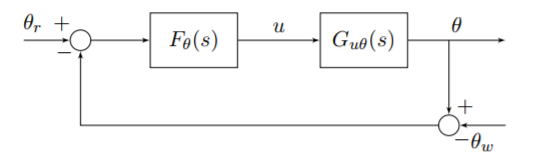
\includegraphics[scale=1]{Figures/blockschema.png}
\caption{ Blockschema vid reglering av vinkeln $\theta$ för roboten.}
\end{figure}\\
Vidare står det i Labb PM:et att överföringsfunktionen för $G_{u \theta}(s)$ är
$$G_{u\theta}(s)=\dfrac{\alpha}{s^2-75.85}=\dfrac{7.55}{s^2-75.85}$$
Blocket $F_\theta(s)$ är systemets regulator med följande regulatorer tillgängliga:\\[0.5em]

$
F_\theta(s)=
\begin{cases}
K_p, \quad \quad \quad \quad \quad \ \ \text{P-regulator}\\[0.5em]
K_p+\dfrac{K_i}{s}, \quad \quad \quad \text{PI-regulator}\\[0.5em]
K_p+\dfrac{sK_d}{1+sT_f},  \ \ \ \text{PD-regulator med LP-filter}
\end{cases}
$ \\[1em]
Systemets kretsöverföring är $L(s)=F_\theta(s)\cdot G_{u \theta}(s)$, detta medför att överföringsfunktionen för det återkopplade systemet blir\\[0.5em]
\begin{equation}
\theta = \dfrac{L(s)}{1+L(s)}\cdot \theta_r
\end{equation}
\subsection{P-regulator}
$L(s) = K_p \cdot \dfrac{7.55}{s^2-75.85}$\\[0.5em]
\begin{flalign*}
\dfrac{\theta}{\theta_r} &= \dfrac{K_p \cdot \dfrac{7.55}{s^2-75.85}}{1+\dfrac{K_p \cdot 7.55}{s^2-75.85}} =\dfrac{K_p \cdot 7.55}{s^2-75.85} \cdot \dfrac{s^2-75.85}{s^2-75.85+K_p\cdot 7.55} = \dfrac{K_p \cdot 7.55 }{s^2-75.85+K_p\cdot 7.55}
\end{flalign*}\\[0.2em]
\begin{tabular}{l|l}
$s^0$&1 \\ 
$s^1$&0\\ 
$s^2$&$C_0$\\
\end{tabular}\\[0.5em]
Utan vidare beräkning kan vi dra slutsatsen att vi inte har alla koefficienter i tabellens första kolumn $(a_0,a_1,c_0,...)$. En P-regulator kan inte detta falla användas för att få samtliga poler i VHP i det återkopplade systemet.
\newpage
\subsection{PI-regulator}
\begin{flalign*}
\dfrac{\theta}{\theta_r} &= \dfrac{L(s)}{1+L(s)}=\dfrac{\bigg (K_p+\dfrac{K_i}{s}\bigg)\cdot \bigg(\dfrac{7.55}{s^2-75.85}\bigg)}{1+\bigg(K_p+\dfrac{K_i}{s}\bigg) \cdot \bigg(\dfrac{7.55}{s^2-75.85}\bigg)} = \dfrac{K_p \cdot 7.55s+K_i\cdot7.55}{s^3-75.85s+K_i \cdot 7.55} &
\end{flalign*}\\[0.2em]
\begin{tabular}{l|l}
$s^0$&$d_0$ \\ 
$s^1$&$c_0$\\ 
$s^2$&0\\
$s^3$& 1 \\
\end{tabular}\\[0.5em]
Vi set att $a_1=0$, med samma argument som för en P-regulator går det inte att implementera en PI-regulator.
\subsection{PD-regulator}
\begin{flalign*}
\dfrac{\theta}{\theta_r} &= \dfrac{L(s)}{1+L(s)} = \dfrac{\bigg(K_p+\dfrac{sK_d}{1+sT_f}\bigg)\cdot \bigg(\dfrac{7.55}{s^2-75.85}\bigg)}{1+\bigg(K_p+\dfrac{sK_d}{1+sT_f}\bigg) \cdot \bigg( \dfrac{7.55}{s^2-75.85}\bigg)}&\\[0.5em]
&=\dfrac{7.55\cdot K_p\cdot (1+sT_f)+K_d \cdot 7.55\cdot s}{s^3\cdot T_f+s^2+(K_p\cdot T_f \cdot 7.55+K_d\cdot 7.55 -75.85\cdot T_f)\cdot s + (K_p \cdot 7.55 - 75.85)}
\end{flalign*}\\[0.2em]
\begin{tabular}{l|l}
$s^0$&$d_0 \quad $ \\ 
$s^1$&$c_0$\\ 
$s^2$&$1 \quad \ \  K_p\cdot7.55-75.85$\\[0.1em]
$s^3$& $T_f \quad K_pT_f\cdot7.55+K_d\cdot7.55-75.85\cdot T_f$ \\
\end{tabular}\\[0.5em]
\begin{flalign*}
C_0 &= \dfrac{a_1a_2-a_3a_0}{a_1} = \dfrac{(K_pT_f\cdot 7.55+K_d\cdot 7.55-75.85\cdot T_f)-(K_pT_f\cdot 7.55-75.85\cdot T_f)}{1}&\\
&=K_d \cdot 7.55 \\[1em]
C_1 &= \dfrac{a_1a_4-a_5a_0}{a_1} =0  &\\[1em]
d_0 &= \dfrac{c_0a_3-c_1a_1}{c_0} = \dfrac{K_d\cdot 7.55 \cdot (K_p \cdot 7.55-75.85)-0}{K_d\cdot 7.55} = K_p \cdot 7.55 - 75.85&\\
\end{flalign*}
Vi får att alla koefficienter i xxx första kolumn är strikt positiva om\\[0.5em]
$
\begin{cases}
T_f>0\\
K_d >0\\
K_p \cdot 7.55 - 75.85 =0 \Rightarrow K_p > \dfrac{1517}{151}
\end{cases}
$
\newpage
\section{Regulatordesign, inre loop}
För att bestämma regulatorparametrarna till PID-regulatorn så att det återkopplade systemet har polerna $-5 \ \pm \ j11, \ -7.5 \ \pm \ j16$ användes programvaran \texttt{Matlab}. Följande värden erhölls\\[1em]
$
\begin{cases}
K_p = 28.5309  \\
K_d = 2.4831 \\
K_i = 241.5285 \\
T_f =  0,0400\\
\end{cases}
$
\newpage
\section{Simulering av den inre balanserande regulatorn}\vspace*{1em}
\begin{enumerate}
\item[a)] Det finns inga anmärkningsvärda skillnader mellan det linjära och olinjära systemet. Det är fullt i linje med våran uppfattning då systemet är linjäriserat avseende på jämviktspunkten d.v.s. när roboten är i ett vertikalt läge.
\item[b)] När det återkopplade systemets mätsignal innehåller störningar sker ett växlande spänningsfall som orsaker problem. Dessa problem inkluderar avläsningsfel som i sin tur leder till att är-värdet (i inre slingan) misstolkas.
\item[c)] 
\end{enumerate}
\newpage
\section{Reglerdesign - Yttre loop}
\begin{figure}[h!]
\centering
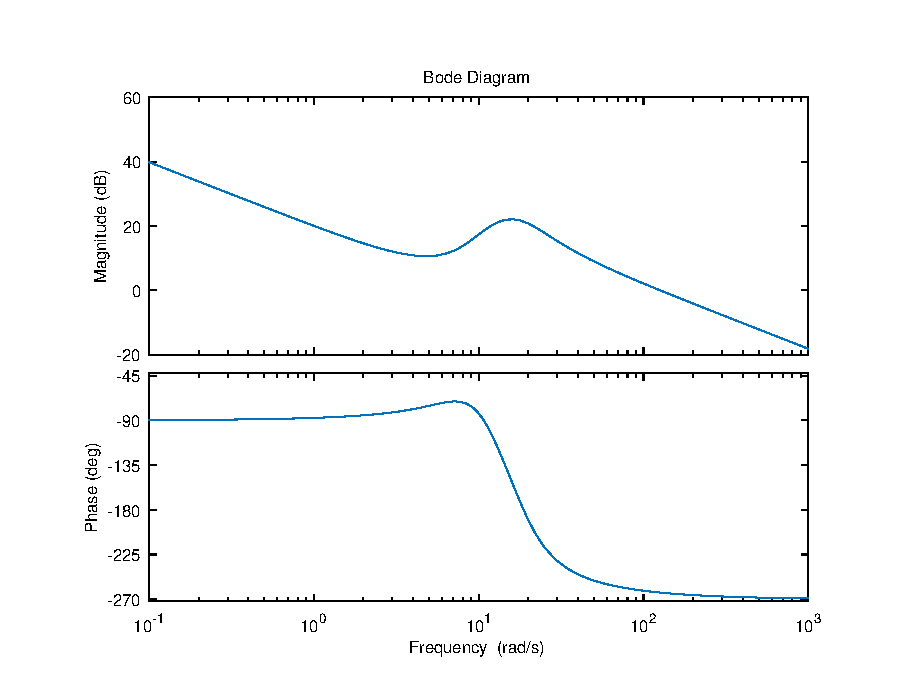
\includegraphics[scale=1]{Figures/bodeplot}
\caption{Bodediagram över processen}
\end{figure}
\newpage
Det skall designas en PI-regulator med som ger en fasmarginal $\varphi = \frac{\pi}{3}$ vid överkorsningsfrekvensen $\omega_c = 0.75 \ rad/s$. Regulatorn har följande parametrisering
\begin{equation*}
\bar{F}_v(s) = K^v_p+\dfrac{K_i^v}{s} = \bigg(1+\dfrac{1}{T_i^vs}\bigg), \quad T_i^v=\dfrac{K_p^v}{K_i^v}.
\end{equation*}
Med önskad fasmarginal $\varphi$ och medföljande överkorsningsfrekvens $\omega_c$ är nästa steg att bestämma $|\bar{F}_v(j\omega_c)|$ samt $\angle \  \bar{F}(j\omega_c)$. Från bodediagrammet (fig. 2) på föregående sida fås
\begin{flalign*}
&arg\{ \bar{F}(j\omega_c)\} = -\tan\bigg(\dfrac{1}{\omega_c T_i^v}\bigg)^{-1} = -180+60-(91.8-180) \approx -31.8^\circ & \\
&\Rightarrow -\tan\bigg(\dfrac{1}{\omega_c T_i^v}\bigg)^{-1}\approx -31.9^\circ, \quad \Rightarrow T_i^v = 2.1338
\end{flalign*}\\[0.5em]
Vidare har vi att
\begin{flalign*}
&|\bar{F}_v(j\omega_c)| = \dfrac{1}{|G_p(j\omega_c)|}=\bigg\{|G_p(j\omega_c)| = 13.2589\bigg\} = \dfrac{1}{13.2589} \approx 0.07542&
\end{flalign*}
och från den givna parametriseringen från labb PM:et fås
\begin{flalign*}
& |\bar{F}_v(j\omega_c)| = K_p^v|1+\dfrac{1}{T_i^vj\omega_c}| = K_p^v\sqrt{1+\bigg(\dfrac{1}{T_i^v\omega_c}\bigg)^2},
\Rightarrow K_p^v = \dfrac{\dfrac{1}{|G_p(j\omega_c)|}}{\sqrt{1+\bigg(\dfrac{1}{T_i^v\omega_c}\bigg)^2}}
\approx 0.06396 &
\end{flalign*}
Vidare finns givet att
\begin{flalign*}
T_i^v=\dfrac{K_p^v}{K_i^v}, \Rightarrow K_i^v=\dfrac{K_p^v}{T_i^v} \approx 0.029975
\end{flalign*}\\[2em]
$
\begin{cases}
K_p^v = -0.06396\\
K_i^v = -0.029975
\end{cases}
$
\newpage
\section{Simulering av det återkopplade systemet}


\end{document}
















